\documentclass[12pt]{article}
\usepackage{makeidx}
\usepackage{multirow}
\usepackage{multicol}
\usepackage[dvipsnames,svgnames,table]{xcolor}
\usepackage{graphicx}
\usepackage{epstopdf}
\usepackage{ulem}
\usepackage{hyperref}
\usepackage{amsmath}
\usepackage{amssymb}
\author{Omkar Mohite}
\title{}
\usepackage[paperwidth=595pt,paperheight=841pt,top=72pt,right=72pt,bottom=72pt,left=72pt]{geometry}

\makeatletter
	\newenvironment{indentation}[3]%
	{\par\setlength{\parindent}{#3}
	\setlength{\leftmargin}{#1}       \setlength{\rightmargin}{#2}%
	\advance\linewidth -\leftmargin       \advance\linewidth -\rightmargin%
	\advance\@totalleftmargin\leftmargin  \@setpar{{\@@par}}%
	\parshape 1\@totalleftmargin \linewidth\ignorespaces}{\par}%
\makeatother 

% new LaTeX commands


\begin{document}


\begin{center}
\textbf{{\LARGE Analysing and Processing Data Packets }}
\end{center}

\begin{enumerate}
	\item \textbf{{\large Tasks to be performed :}}
	\begin{itemize}
	\item Pairing EEG sensor with laptop using JY-MCU bluetooth module.
	\item Observing and analysing Data packets and processing it.
	\item Connection of Bluetooth on the Firebird V.
	\item Pairing Neurosky EEG sensor with Firebird V.
	\end{itemize}



	\item \textbf{{\large Pairing EEG sensor with laptop using JY-MCU bluetooth module:}}


In the last tutorial we have seen how to give configure bluetooth module using
AT commands. In the similar manner we have to observe data packets which are send
by Neurosky Mindwave Headset.

\begin{enumerate}
\item \textbf{Connections:}

\begin{itemize}
	\item Connect the bluetooth module to USB to serial converter as performed while giving AT commands.
	\item As the bluetooth module is configured and bound with Mindwave headset. Pair the module with sensor.
	\item How to Pair Mindwave mobile headset?\\
	Press up the button on the side of headset to turn it on. Blinking of blue light once indicates that it is turned on. Now again press up the button and keep pressing until it starts blinking twice. Now it has gone in finding devices. As the passcode set of bluetooth module and headset is same ie. 0000. It will pair with each other. On the headset continuos blue light indicates it has paired with the bluetoth module. Red light blinking on headset indicates it has went in reset mode.
	

	\item Once you have paired with the device now you can observe data values coming from sensor.
\end{itemize}
\end{enumerate}


	\item \textbf{{\large Observing and analysing Data packets and processing it:
			}}


To observe the data values on the screen of you laptop, make use of terminal named '\textbf{Realterm}'\\\\\\\\\\\\\\\\\\\\\\\\.

\begin{center}
\textbf{Fig 1: }Realterm terminal screenshot
	\graphicspath{ {images/} }
	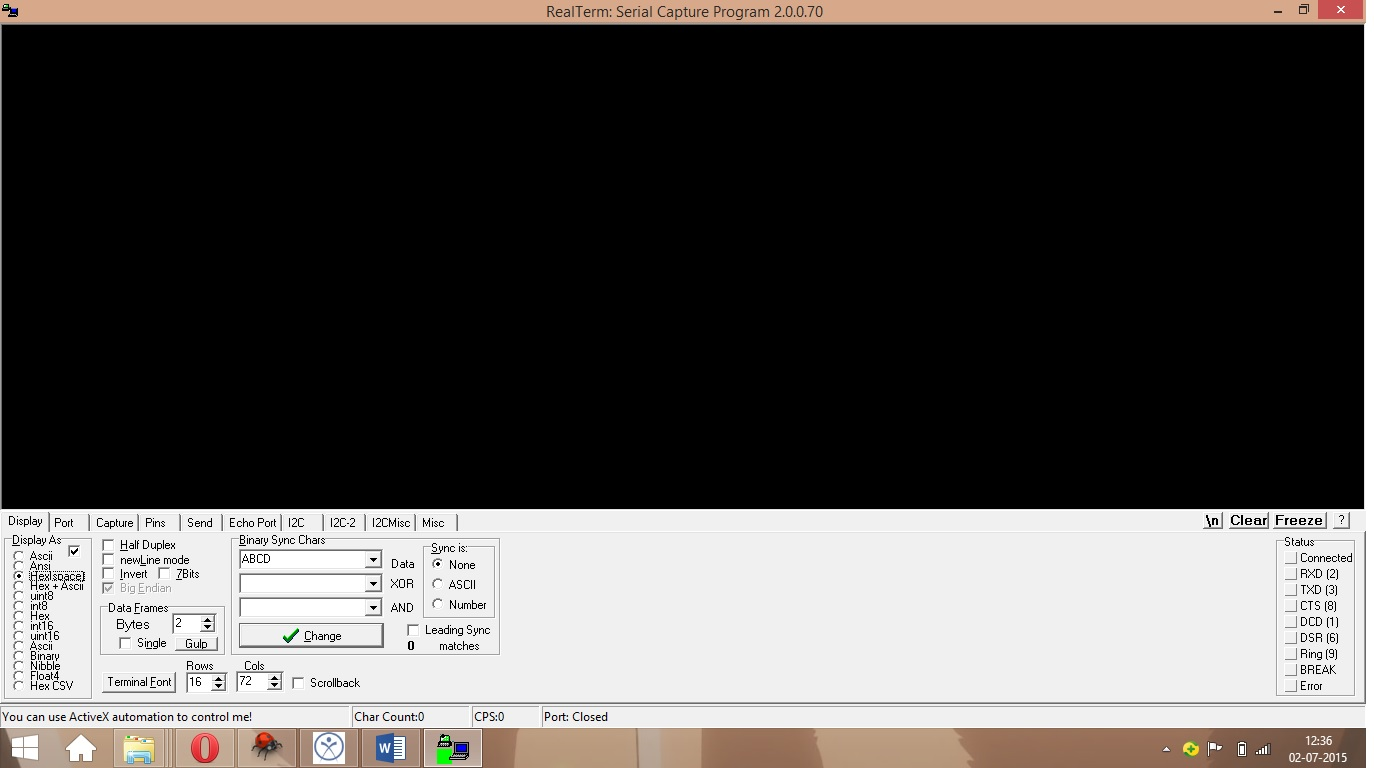
\includegraphics[width=11.5cm, height=7cm]{Realterm}
\end{center}
\begin{enumerate}
	\item \textbf{Settings:}

\begin{itemize}
	\item Open Realterm.
	\item Go to diplay section and select Display as `Hexlspace'.
	\item Go to ‘Port’ section and set baud rate as 9600, stop bit 1, start bit 0. Now once you have paired the device properly go to ‘Port’ section and click open. 
	\item You will see continuous data stream coming on the terminal.
\end{itemize}


	\item \textbf{Analysing data packets:}


\begin{itemize}
	\item As we know data packet structure covered in Tutorial on Neurosky Mindwave mobile Headset. The data packet has two SYNC bytes ‘AA’. Then has another byte which is Payload Length and further consists of Payload data bytes and number of payload data bytes depend upon payload length.
	\item The last byte of the packet is checksum byte. We have to verify checksum byte and confirm about the obtained data packets whether they are accurate or not.\\\\\\\\\\\\\\\\\\\\\\\\\\
\end{itemize}

\begin{center}
\textbf{Fig  2.} Data values obtained:
	\graphicspath{ {images/} }
	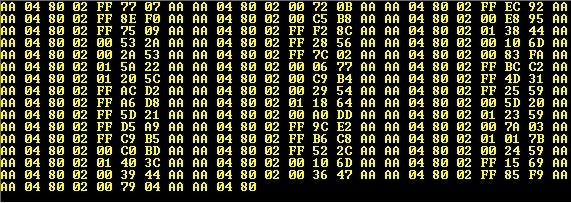
\includegraphics[width=15cm, height=6.6cm]{data_values}
\end{center}
	\item \textbf{Processing Data Packets:}

\begin{center}
	\textbf{Fig 3:}Processing Data values
	\graphicspath{ {images/} }
	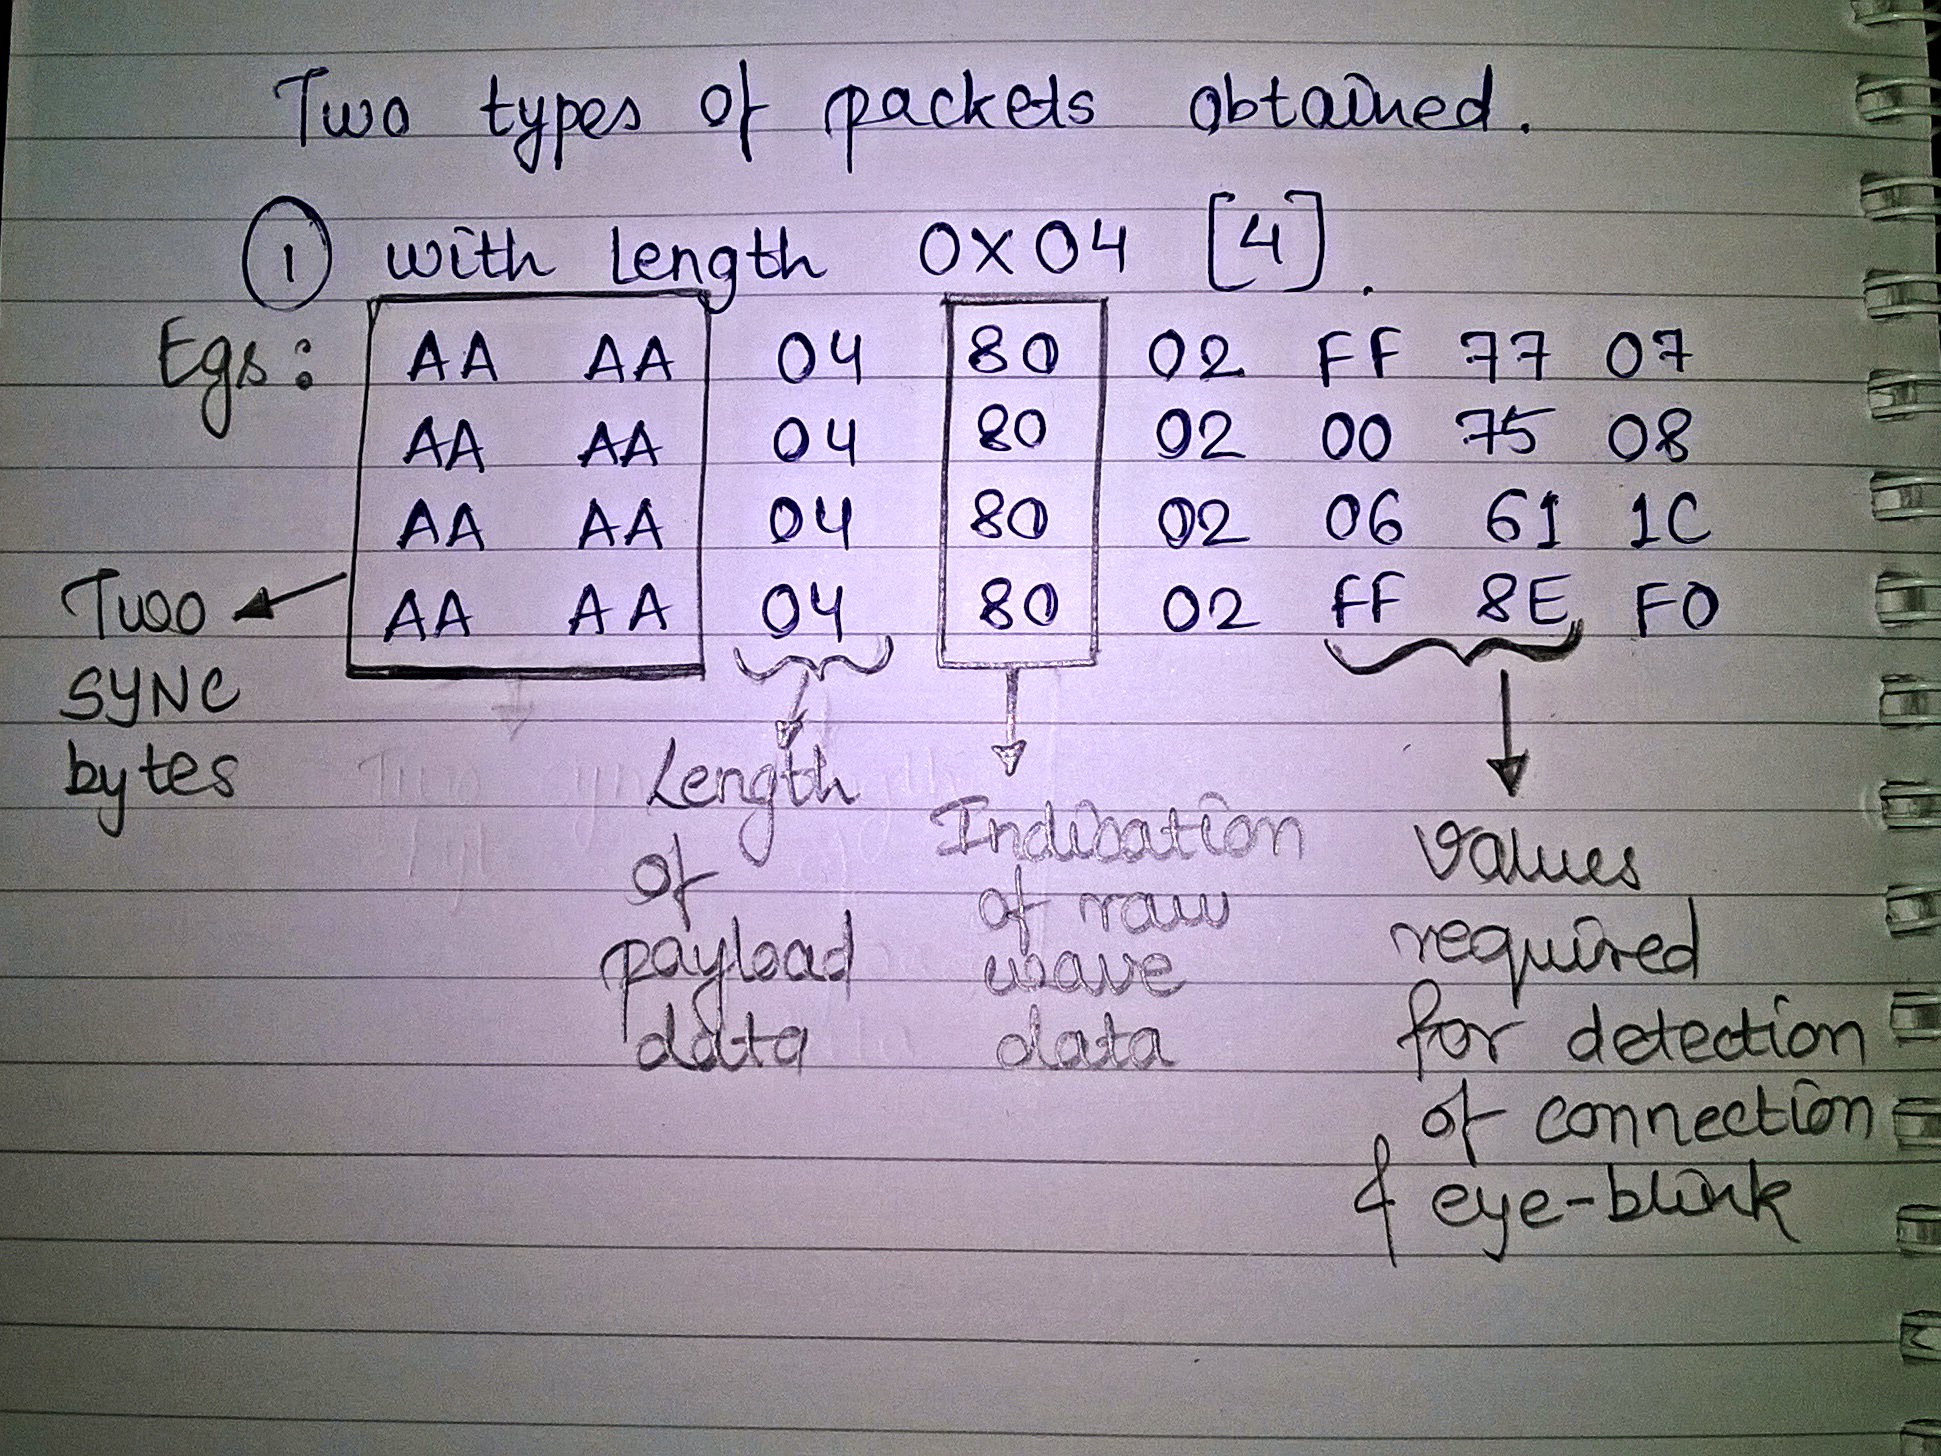
\includegraphics[width=15cm, height=10cm]{Process1}
\end{center}
\begin{itemize}
	\item As you can see the above image of the processed data. We obtain only two types of data packets. Payload length of 0x04 and 0x20. 
	\item The 0x04 payload length data packet consists of raw values which indicates mainly the connection of headset on head, pairing values, and eye-blink data values which are send when scalp touched to cathode and anode are moved.
	\item The 0x20 payload length data packet consists of poor quality indication, attention level indication and meditation level indication.
	\item 0x02 indicates poor quality detection. The next byte to that indicates poor quality signal level. For eye-blink detection this value should be 0.
	\item 0x04 indicates attention level detection. The next byte to that indicates level of attention.
	\item 0x05 indicates meditation level detection. The byte next to 0x05 indicates meditation level achieved.
	\item 0x02 always appear next to 0x20 i.e. next to payload length.
	\item 0x04 always appear at 28$^{th}$ position of payload data and 0x05 always appear
at 30$^{th}$ position of payload data.
	\item For attention, meditation and poor quality detection 0x20 byte long payload data is useful.
	\item For eye-blink detection 0x04 byte long payload data is useful.
\end{itemize}
\end{enumerate}

\begin{center}
	\textbf{Fig 4: }Processing Data values
	\graphicspath{ {images/} }
	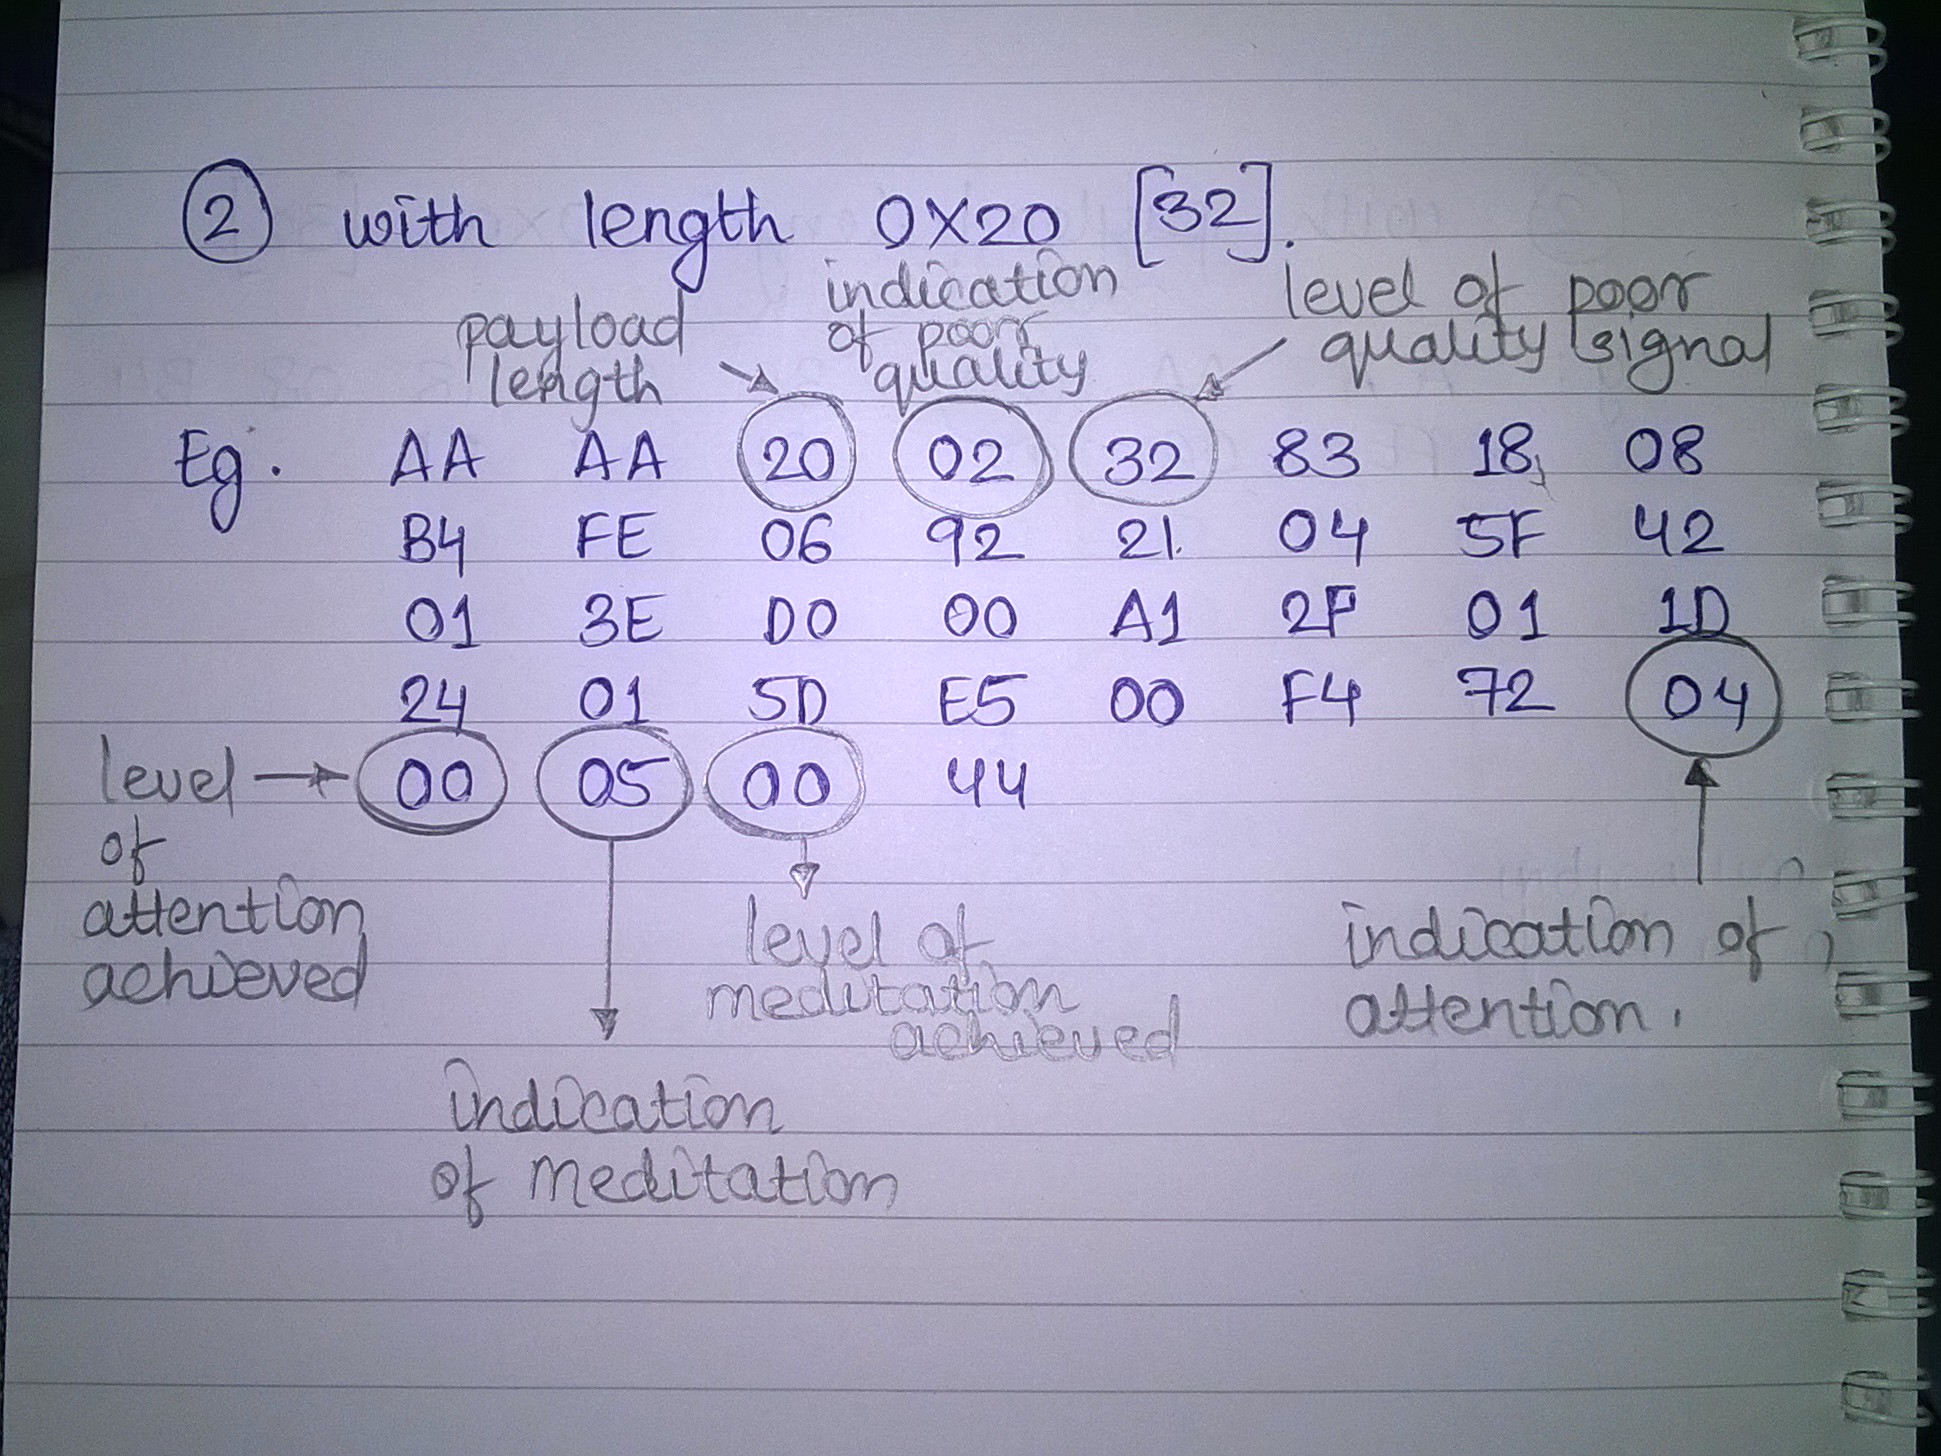
\includegraphics[width=15cm, height=10cm]{Process2}
\end{center}

	\item \textbf{{\large Pairing Neurosky EEG sensor with Firebird V.}}
	\begin{itemize}
	\item Connect Bluetooth on Firebird V.
	\item Make use of expansion slot of UART connections.
	\item Connect to 37 and 38 pin no. of expansion slot. 37 pin no. indicates TXD and 38 pin no. indicates RXD.
	\item Connect RXD of bluetooth module to TXD of Firebird V and vice versa.
	\item Connect VCC to pin no.1 of and GND to pin no.2 of expansion slot.
	\item Now pair your headset with bluetooth module as explained above.
	\item Load your program for normal data receiving and observe the changes on bot according to the data received from the sensor.\\
\end{itemize}
\end{enumerate}

\textbf{{\large References:}}

\begin{itemize}
	\item MindGear headset datasheet. (uploaded in datasheets folder in github link)
	\item Hardware and software manual of Firebird V uploaded in datasheets and manuals folder.
\end{itemize}


\end{document}